\documentclass{standalone}
\usepackage{graphicx}	
\usepackage{amssymb, amsmath}
\usepackage{color}

\usepackage{tikz}
\usetikzlibrary{intersections, backgrounds}
\usepackage{pgfmath}

\definecolor{light}{RGB}{220, 188, 188}
\definecolor{mid}{RGB}{185, 124, 124}
\definecolor{dark}{RGB}{143, 39, 39}
\definecolor{highlight}{RGB}{180, 31, 180}
\definecolor{gray10}{gray}{0.1}
\definecolor{gray20}{gray}{0.2}
\definecolor{gray30}{gray}{0.3}
\definecolor{gray40}{gray}{0.4}
\definecolor{gray60}{gray}{0.6}
\definecolor{gray70}{gray}{0.7}
\definecolor{gray80}{gray}{0.8}
\definecolor{gray90}{gray}{0.9}
\definecolor{gray95}{gray}{0.95}

\newcommand*{\offset}{0.025}

\begin{document}

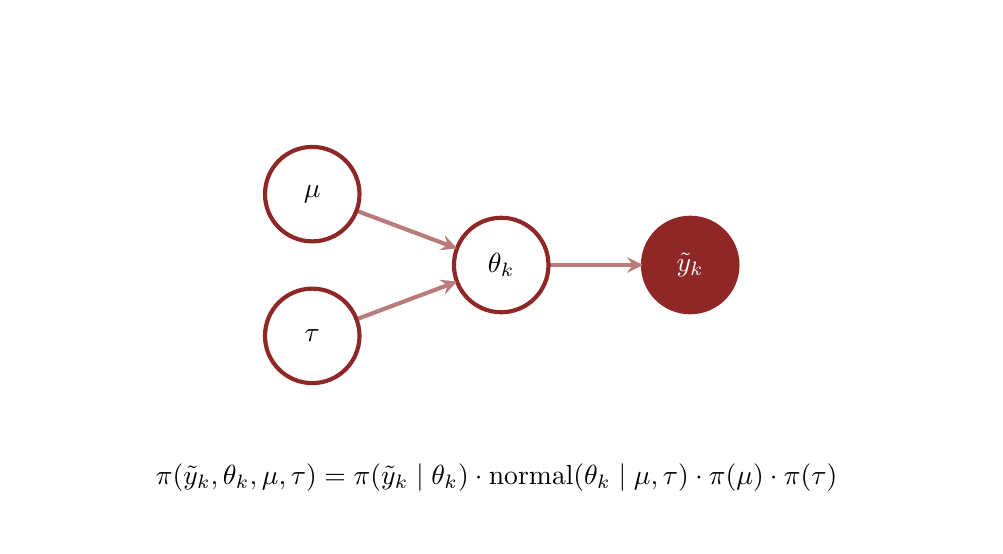
\begin{tikzpicture}[scale=0.3, thick]

\pgfmathsetmacro{\r}{2}

\pgfmathsetmacro{\dx}{0}
\pgfmathsetmacro{\dy}{0}

\draw[white] (-20 + \dx, -11 + \dy) rectangle (20 + \dx, 10 + \dy);

\node[align=center] at (0 + \dx, -9 + \dy) 
{ $ \pi (\tilde{y}_{k}, \theta_{k}, \mu, \tau) = \pi (\tilde{y}_{k} \mid \theta_{k} ) \cdot \text{normal}(\theta_{k} \mid \mu, \tau)
\cdot \pi (\mu) \cdot \pi (\tau) $ };

\filldraw[fill=dark, draw=dark, line width=1.5] (8 + \dx, 0 + \dy) circle (\r)
node[color=white] { $\tilde{y}_{k}$ };

\draw[->, >=stealth, color=mid, line width=1.5] 
  ({0 + \r + \dx}, {0 + \dy}) -- ({8 - \r + \dx}, {0 + \dy});

\filldraw[fill=white, draw=dark, line width=1.5] (0 + \dx, 0 + \dy) circle (\r)
node[color=black] { $\theta_{k}$ };

\draw[->, >=stealth, color=mid, line width=1.5] 
  ({-8 + \r * cos(20.56) + \dx}, {3 - \r * sin(20.56) + \dy}) -- ({0 - \r * cos(20.56) + \dx}, {0 + \r * sin(20.56) + \dy});

\filldraw[fill=white, draw=dark, line width=1.5] (-8 + \dx, 3 + \dy) circle (\r)
node[color=black] { $\mu$ };

\draw[->, >=stealth, color=mid, line width=1.5] 
  ({-8 + \r * cos(20.56) + \dx}, {-3 + \r * sin(20.56) + \dy}) -- ({0 - \r * cos(20.56) + \dx}, {0 - \r * sin(20.56) + \dy});

\filldraw[fill=white, draw=dark, line width=1.5] (-8 + \dx, -3 + \dy) circle (\r)
node[color=black] { $\tau$ };

\end{tikzpicture}

\end{document}  